\documentclass[onecolumn, draftclsnofoot,10pt, compsoc]{IEEEtran}
\usepackage{graphicx}
\usepackage{url}
\usepackage{setspace}
\setlength\parindent{0pt}
\usepackage{geometry}
\usepackage{minted} % code highlighting
\usepackage{listings} % fallback code highlighting
\usepackage{xcolor}
\usepackage{tabularx}
\usepackage{longtable}
\geometry{textheight=9.5in, textwidth=7in}

% define code snippet styles

\graphicspath{{./images/}}

\definecolor{codegreen}{rgb}{0,0.6,0}
\definecolor{codegray}{rgb}{0.5,0.5,0.5}
\definecolor{codepurple}{rgb}{0.58,0,0.82}
\definecolor{backcolour}{rgb}{0.95,0.95,0.92}

\lstdefinestyle{mystyle}{
    backgroundcolor=\color{backcolour},   
    commentstyle=\color{codegreen},
    keywordstyle=\color{magenta},
    numberstyle=\tiny\color{codegray},
    stringstyle=\color{codepurple},
    basicstyle=\ttfamily\footnotesize,
    breakatwhitespace=false,         
    breaklines=true,                 
    captionpos=b,                    
    keepspaces=true,                 
    numbers=left,                    
    numbersep=5pt,                  
    showspaces=false,                
    showstringspaces=false,
    showtabs=false,                  
    tabsize=2
}

\lstset{style=mystyle}

% 1. Fill in these details
\def \CapstoneTeamName{		BBM}
\def \CapstoneTeamNumber{		26}
\def \GroupMemberOne{			Aidan Grimshaw}
\def \GroupMemberTwo{			Khoa Tran}
\def \GroupMemberThree{			Aaron Leenknecht}
\def \CapstoneProjectName{		Baby Body Measurement Using Computer Vision}
\def \CapstoneSponsorPerson{		D. Kevin McGrath}

% 2. Uncomment the appropriate line below so that the document type works
\def \DocType{		%Problem Statement
				%Requirements Document
				% Technology Review
				%Design Document
				Winter Term Progress Report
				}
			
\newcommand{\NameSigPair}[1]{\par
\makebox[2.75in][r]{#1} \hfil 	\makebox[3.25in]{\makebox[2.25in]{\hrulefill} \hfill		\makebox[.75in]{\hrulefill}}
\par\vspace{-12pt} \textit{\tiny\noindent
\makebox[2.75in]{} \hfil		\makebox[3.25in]{\makebox[2.25in][r]{Signature} \hfill	\makebox[.75in][r]{Date}}}}
 %3. If the document is not to be signed, uncomment the RENEWcommand below
\renewcommand{\NameSigPair}[1]{#1}

%%%%%%%%%%%%%%%%%%%%%%%%%%%%%%%%%%%%%%%
\begin{document}
\begin{titlepage}
    \pagenumbering{gobble}
    \begin{singlespace}
    %	
\includegraphics[height=4cm]{coe_v_spot1}
        \hfill 
        % 4. If you have a logo, use this includegraphics command to put it on the coversheet.
        %\includegraphics[height=4cm]{CompanyLogo}   
        \par\vspace{.2in}
        \centering
        \scshape{
            \huge CS Capstone \DocType \par
            {\large\today}\par
            \vspace{.5in}
            \textbf{\Huge\CapstoneProjectName}\par
            %\vspace{.7in}
            \vspace{10mm}
            %\vfill
            {\large Prepared for}\par
            \vspace{5mm}
            % \Huge \CapstoneSponsorCompany\par
            %\vspace{5mm}
            {\Large\NameSigPair{\CapstoneSponsorPerson}\par}
            \vspace{5mm}
            {\large Prepared by }\par
            \vspace{5mm}
            Group\CapstoneTeamNumber\par
            % 5. comment out the line below this one if you do not wish to name your team
            \CapstoneTeamName\par 
            \vspace{5pt}
            {\Large
                %\NameSigPair{\GroupMemberOne}\par
                %\NameSigPair{\GroupMemberTwo}\par
                %\NameSigPair{\GroupMemberThree}\par
                
                \GroupMemberOne\par
                \GroupMemberTwo\par
                \GroupMemberThree\par
            }
            \vspace{.8in}
        }
        \begin{abstract}
            This document chronicles and details the team's progress by the end of Winter Term of 2020. It also briefly recaps the projects current state and what steps are left until completion.
        \end{abstract}     
    \end{singlespace}
\end{titlepage}
\newpage
\pagenumbering{arabic}
\tableofcontents
% 7. uncomment this (if applicable). Consider adding a page break.
%\listoffigures
%\listoftables
\clearpage



\section{Project's Purposes and Goals}
The project involves designing an iOS application that uses computer vision to measure a baby's body. The users goal will be to take measurements of their baby with an emulated tape measure through their phone's camera. Taking a measurement through the phone satisfies the purpose of being able to accurately and easily measure a baby from their residence without the need to visit the doctor's office. A goal of the application is to store all measurements taken and to display that information in a meaningful manner. All health information will be pulled from the World Health Organization to make sure of its accuracy.


\section{Current Progress}
The application consists of four aspects:\par
\begin{itemize}
    \item Traversal of the application - Beta Level Completion
    \vspace{2}
    \item Storing/Receiving data - Beta Level Completion
    \vspace{2}
    \item Taking the measurement - Beta Complete Completion
    \vspace{2}
    \item Displaying/Explaining the measurements - Beta Level Completion\\
\end{itemize}

The user starts out on the home page of the application which consists of a baby selection and four other buttons. A picker wheel is used to select the baby that the user wants to continue the application with and is populated with baby profiles that have already been created. The picker wheel is dynamically linked to the Core Data database to populate it automatically. The first button will lead to a profile creation screen. The second button takes the user to the measurement screen. The third button brings the user to a menu that has a list of buttons to take the user to different graphs. The fourth button takes the user to an informational screen. Currently, the home page and the profile creation page are completely finished. In the profile creation page, there are five user inputs that the application gathers: first name, last name, date of birth, biological sex, and height when born. All inputs on the profile creation screen are constrained with date pickers, two item selectors, and units given to prevent user error. There is a save button at the bottom of the profile creation screen that takes all the values that have been inputted and stores them in the Core Data database under that specific child. On the measurement page, the user can add points to the screen which will gather a measurement between two points. It currently has a save button that will save the measurement between two points as the baby's height in the database for the specific child. The graph menu page currently has two buttons that lead to separate graphs for visualizing measurement data. One visualization option is a bar graph that displays recent measurements. The other is a comparative line chart which takes in recent measurements and compares those to the 1st and 99th percentile of babies of similar gender over the first 12 months of age. On the information page it retrieves data from the Core Data database including: most recent height, height when born, name, and date of birth. It uses that data to display the following information to the user: name, height, height they've grown since birth, the percentile their height falls in comparative to other babies, and how many weeks old they are.


\section{What's Left}
\begin{itemize}
    \item We have to fix a bug with persisting the selected child on the home screen. Right now if a child is selected and a button is pushed to go to a different screen, that child shows up. However, if the user goes back to the main menu with the child selected and chooses a different screen, the first child is passed in rather than the selected child.\\

    \item The value of the measurement is displayed on screen in meters. We want to plug in a formula to change that value to display in inches to the user.\\

    \item On the informational page, we want to incorporate the baby's percentile and what that means according to the World Health Organization. Different levels of percentiles mean different things, such as start feeding them formula over breast milk, be worried or not worried, etc.\\
    
    \item Additionally, UI improvement is sorely needed on the information page. Currently, it only displays plain text, all of which is centered on the screen. We'd like to align elements better and add colors to the percentile field to indicate baby's health. For example, a percentile of less than 25\% is colored red to warn the parent that their baby may be growing below average.
    
    \item Polishing all aspects will take place. Making sure text fields, buttons, etc. are all placed and sized the best possible way with constraints in place for responsive design.\\
    
    \item Adding the delete profile option to the home menu. This will be beneficial to development as well as the user if they make a mistake in the profile creation screen.\\
    
    \item Add a constraint feature that greys out the save button when creating a profile until all fields are filled in.\\
    
    \item Add more customizable features to the comparative line chart so the user can see different data in different ways.\\
\end{itemize}


\section{Problems & Solutions}

We ran into issues with finding a good charting library. Our application is being built using storyboard, which is an older IOS UI framework. We did this in order to make ARKit work correctly in the application. However, there are less charting frameworks available for this.\\

We also struggled with installing and using the charting library available. We initially installed the charting library by copying in the charting library repository, but this was obviously not a solution that would work long term. We decided to transfer to using the package manager cocoapods to manage this dependency.\\

Initially the plan was to incorporate Apple's body height estimation so the measurements could be taken in an 'automatic' manner. After attempting to integrate that technology into our project, we figured out that the documentation online was different than the documentation within the project's repository. Our solution was to fully switch measurement techniques to model the idea of a tape measure. A tape measure allows the user to get whatever measurement they would like.\\

Finally we struggled with implementing proper time scaling of the graph data points. Our scale was in months but our data needed to be in days to allow for interpolation between months. To solve this problem, the days since birth were divided 30 to get a rough estimation of where they were on a month scale, since the average number of days in a month is 30. This scale doesn't need to be incredibly accurate since children will not change in height much from day to day, but it does need to have some degree of accuracy.


\section{Interesting Code}

The application records coordinates in the world by performing a "hit test". A "hit test" determines whether the touch location is on a feature point, i.e. point detected in the augmented world.

\begin{lstlisting}[swift, caption={Hit test}]
override func touchesBegan(_ touches: Set<UITouch>, with event: UIEvent?) {
    // record at most two points
    if dotNodes.count >= 2 {
        for dot in dotNodes {
            dot.removeFromParentNode()
        }
        dotNodes = [SCNNode]()
    }
    
    if let touchLocation = touches.first?.location(in: sceneView) {
        // perform hit test
        let hitTestResults = sceneView.hitTest(touchLocation, types: .featurePoint)
        // if a feature point is hit, record it
        if let hitResult = hitTestResults.first {
            addDot(at: hitResult)
        }
        
    }
}
\end{lstlisting}

The point is then used to contruct a 3D SceneKit vector to be rendered in the AR view:

\begin{lstlisting}[swift, caption={Construct 3D vector}]
let dotNode = SCNNode(geometry: dotGeometry)
// construct a 3D vector
dotNode.position = SCNVector3(hitResult.worldTransform.columns.3.x, hitResult.worldTransform.columns.3.y, hitResult.worldTransform.columns.3.z)

sceneView.scene.rootNode.addChildNode(dotNode)
\end{lstlisting}

Once two points are recorded, the distance between them is calculated using the Pythagorean theorem:

\begin{lstlisting}[swift, caption={Pythagorean theorem}]
func calculate () {
    let start = dotNodes[0]
    let end = dotNodes[1]
    
    // Apply Pythagorean theorem on start and end points
    let distance = Double(
        sqrt(
            pow(end.position.x - start.position.x, 2) +
            pow(end.position.y - start.position.y, 2) +
            pow(end.position.z - start.position.z, 2)
        )
    )
}
\end{lstlisting}


\section{Screenshots of Project}

\begin{figure}[h!]
\centering
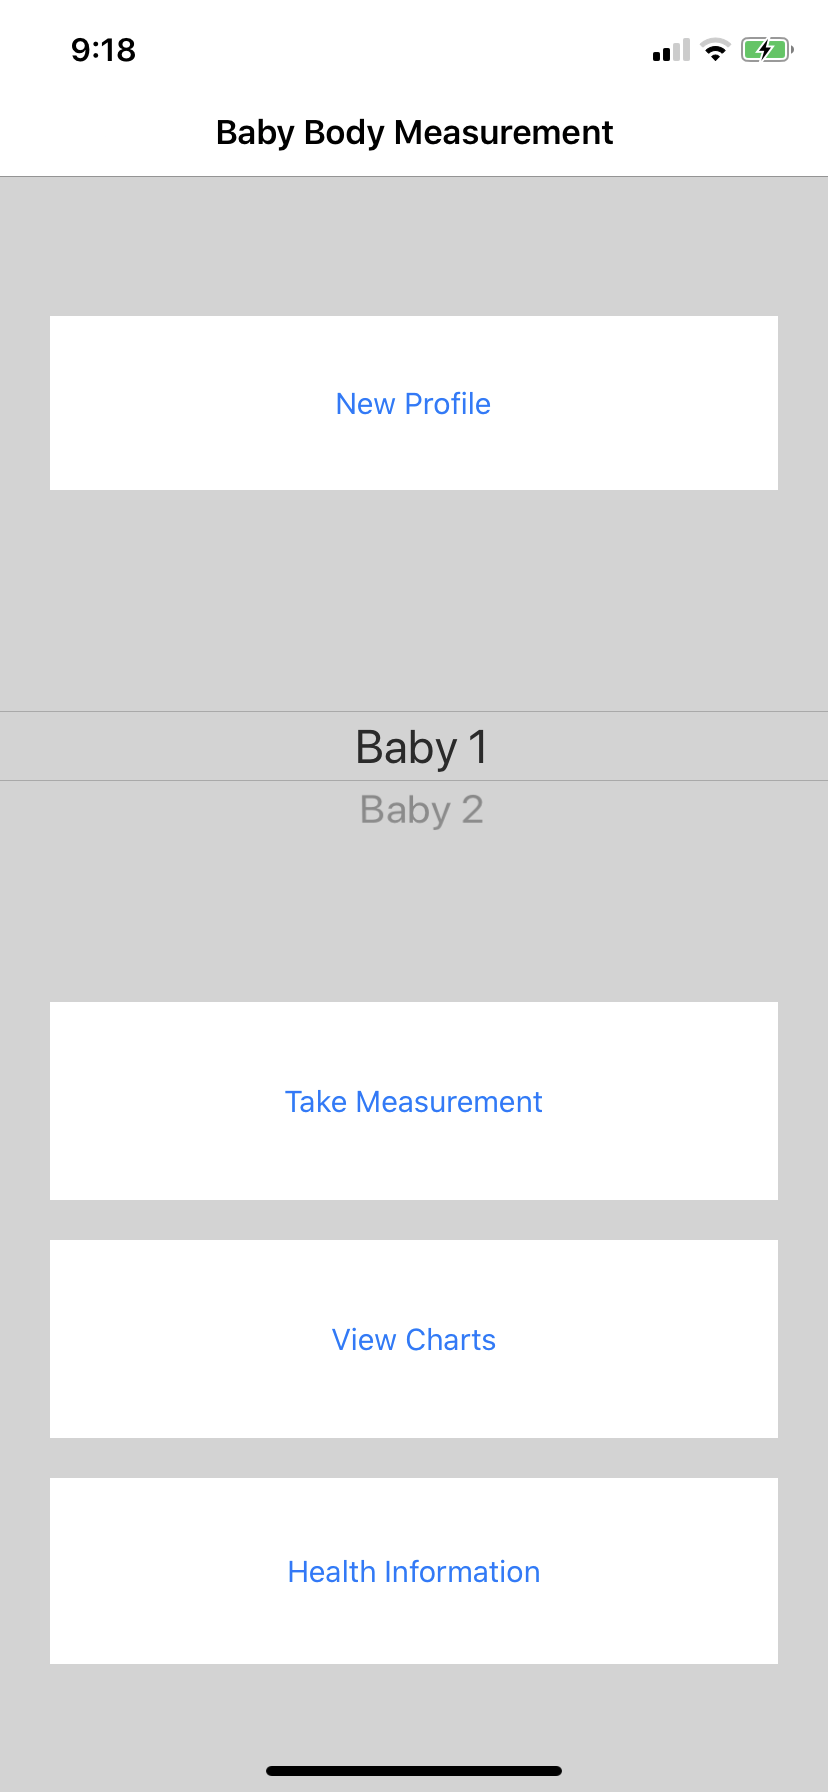
\includegraphics[width=70mm]{./images/home-screen.png}
\caption{Home screen}
\end{figure}

\begin{figure}[h!]
\centering
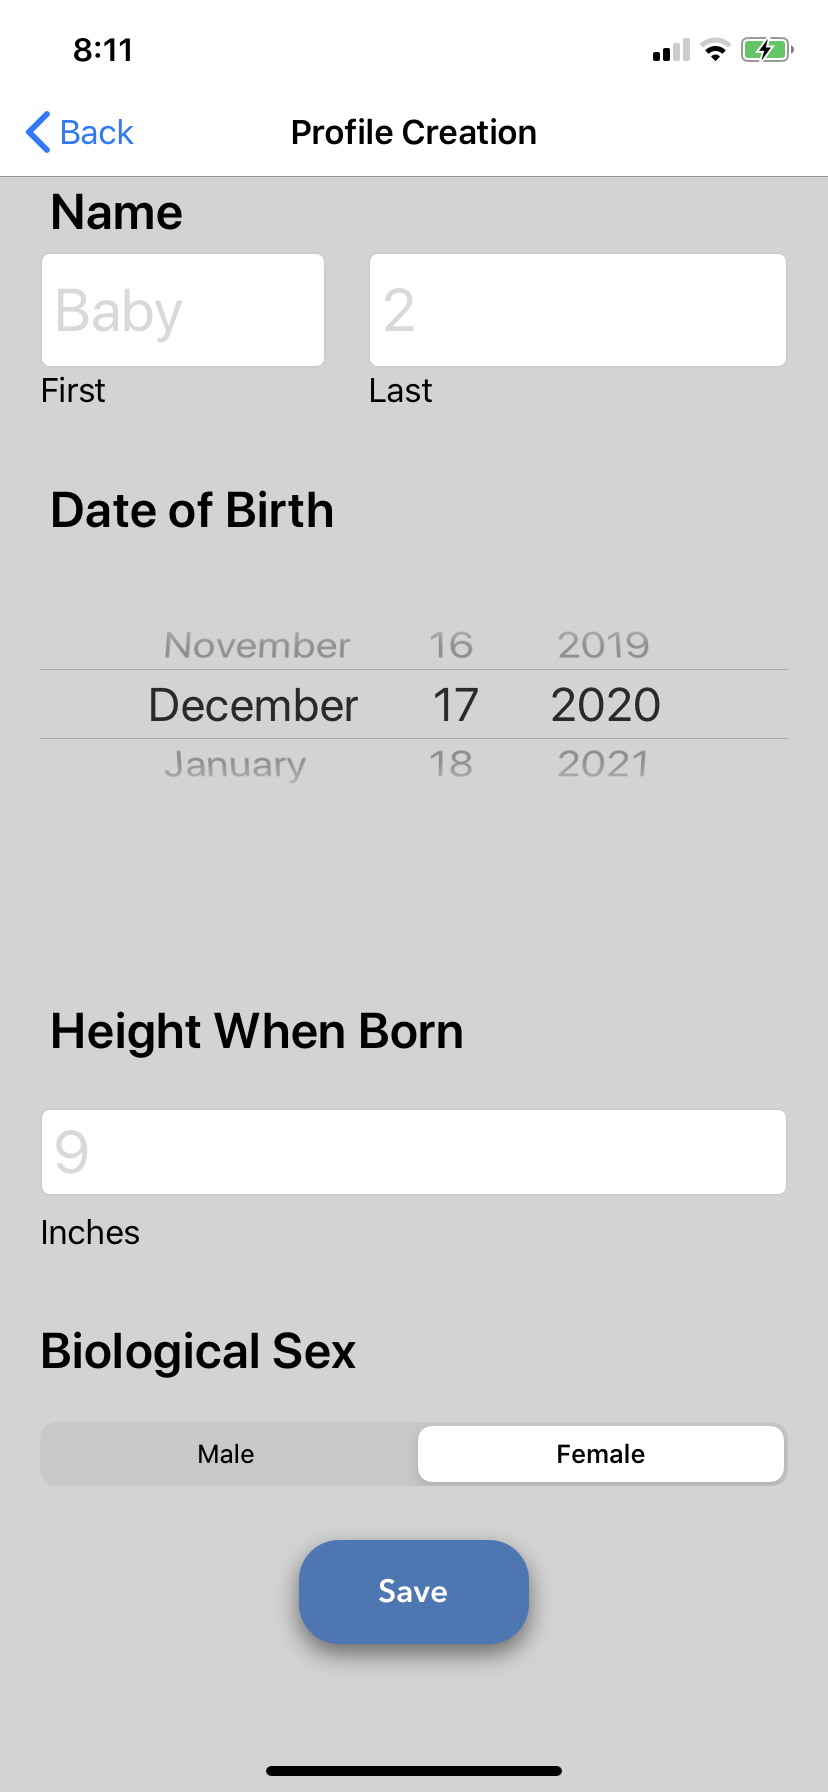
\includegraphics[width=70mm]{./images/new-profile-screen.png}
\caption{New profile screen}
\end{figure}

\begin{figure}[h!]
\centering
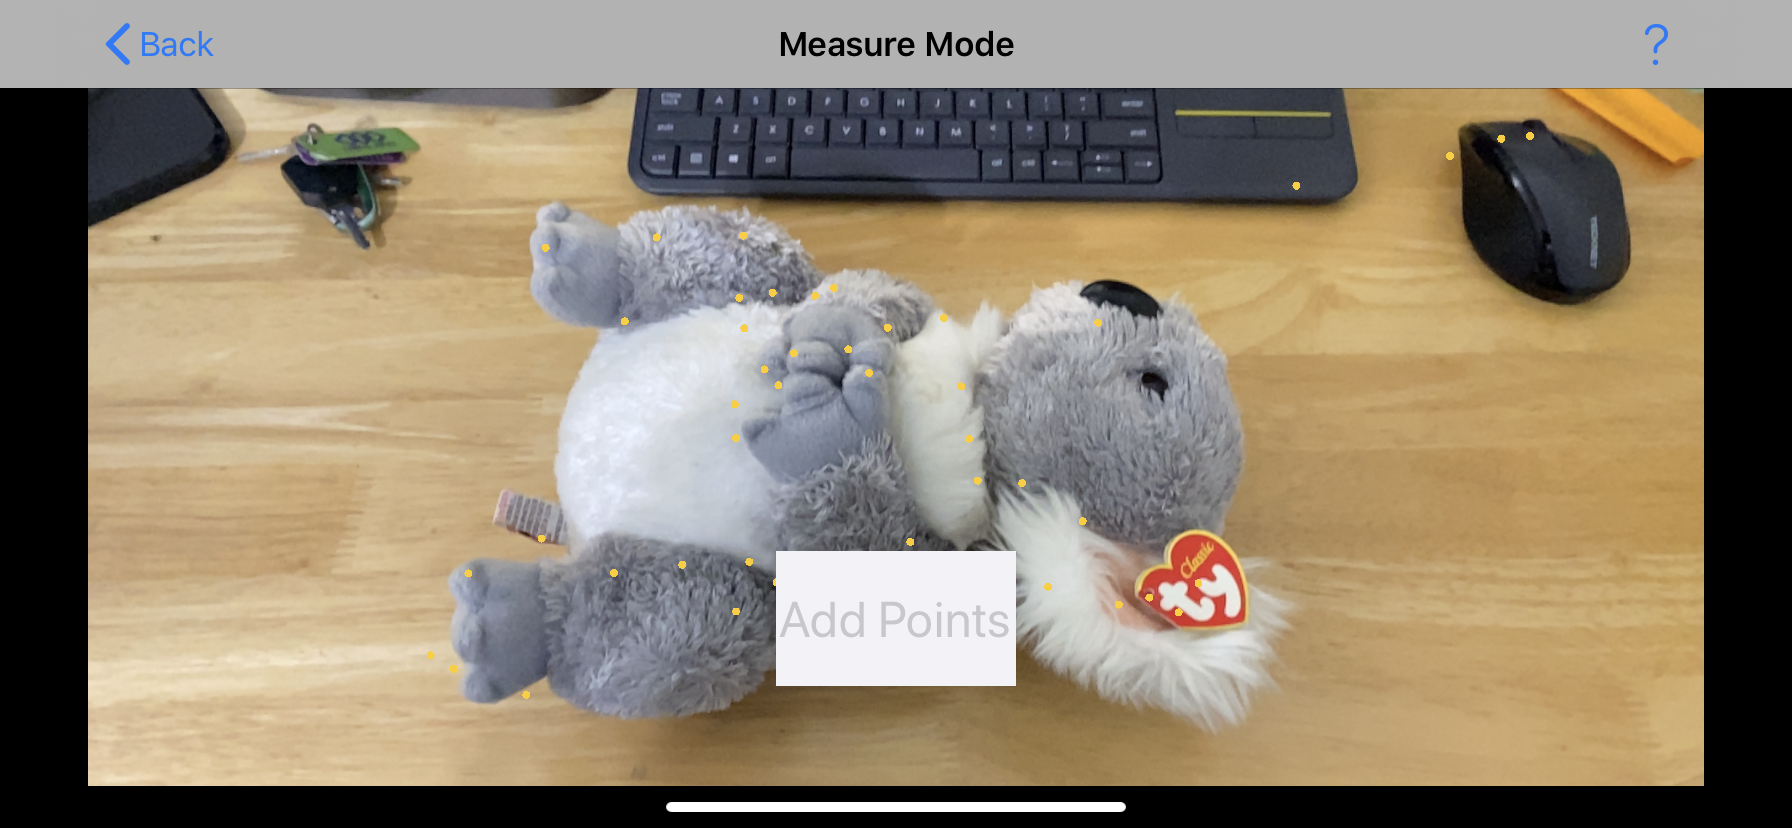
\includegraphics[width=70mm]{./images/measure-screen.png}
\caption{Measure screen}
\end{figure}

\begin{figure}[h!]
\centering
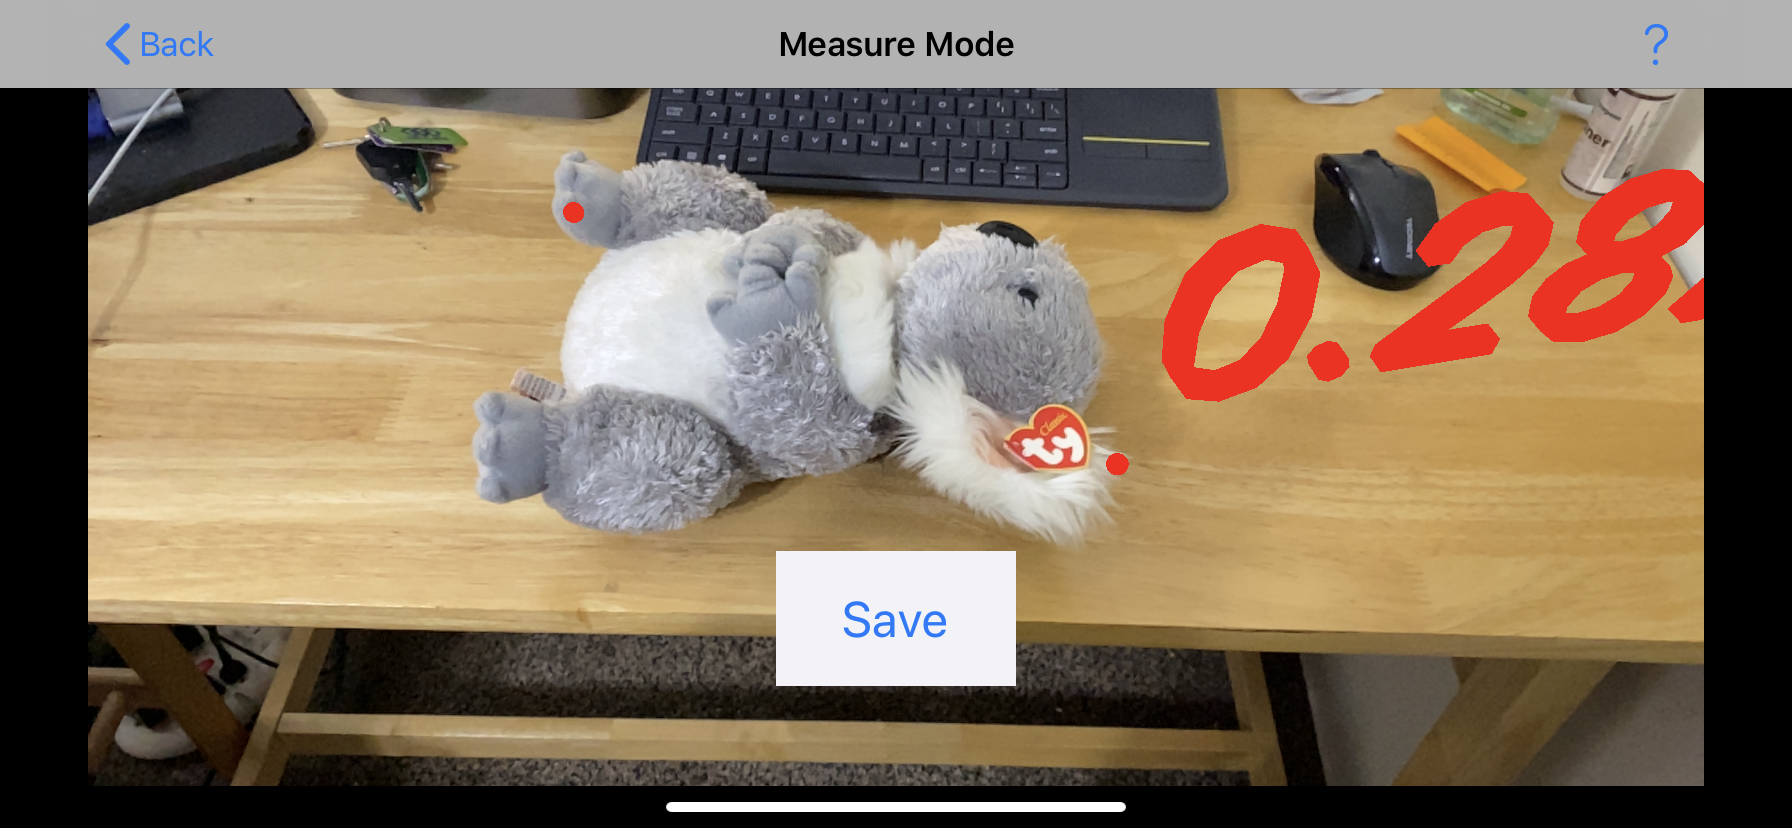
\includegraphics[width=70mm]{./images/measure-points-screen.png}
\caption{Measure screen with points}
\end{figure}

\begin{figure}[h!]
\centering
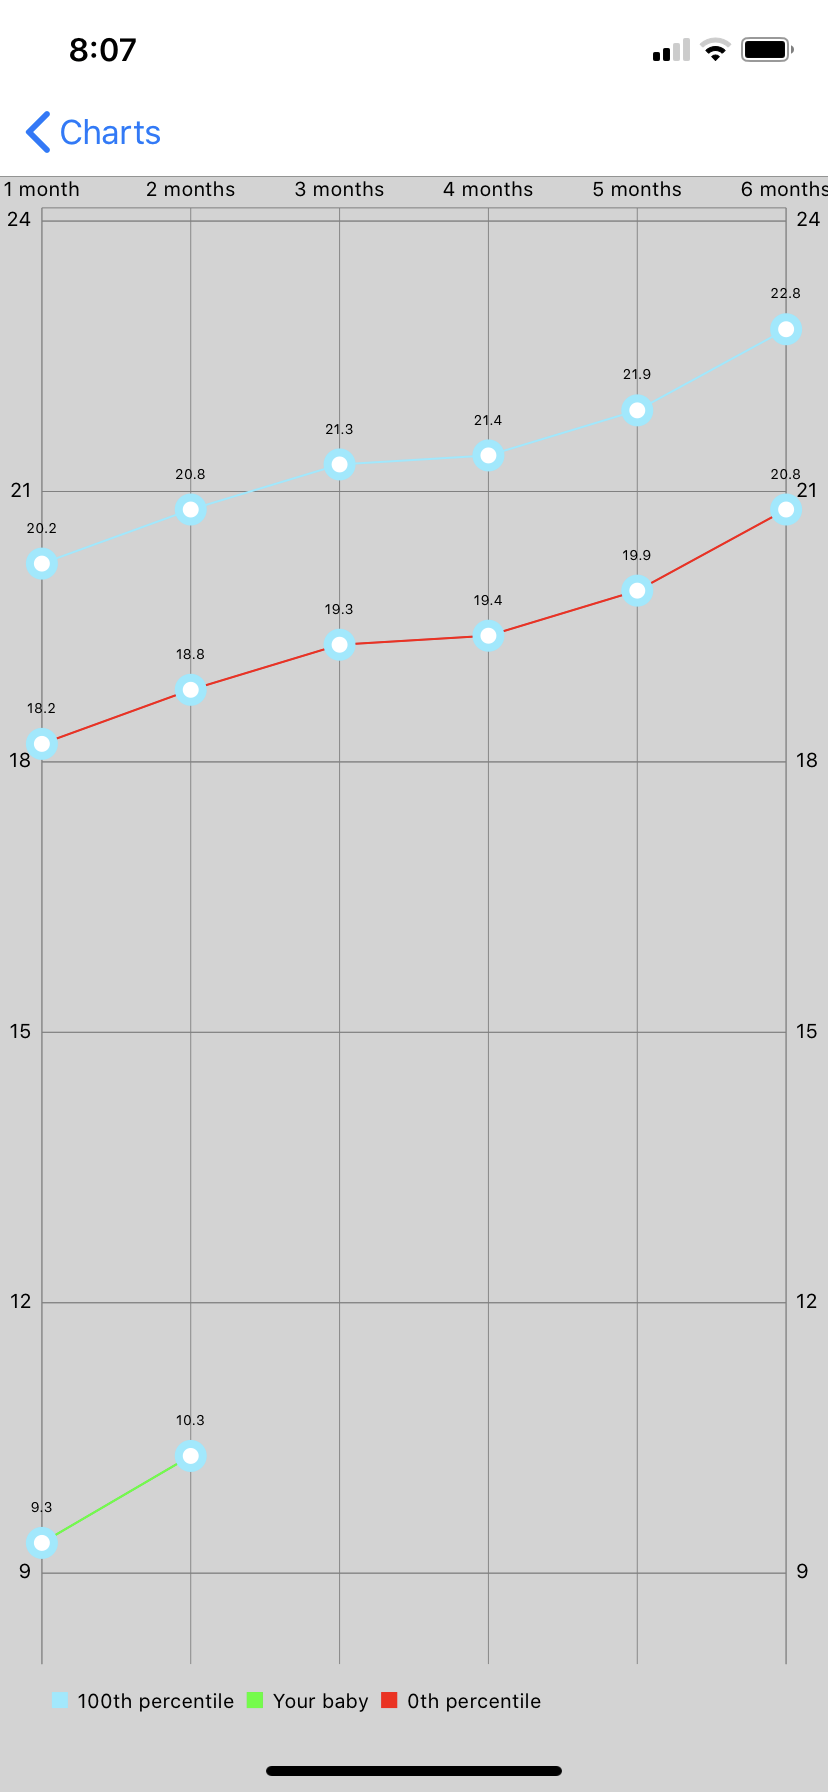
\includegraphics[width=70mm]{./images/line-graph-screen.png}
\caption{Line graph screen}
\end{figure}

\begin{figure}[h!]
\centering
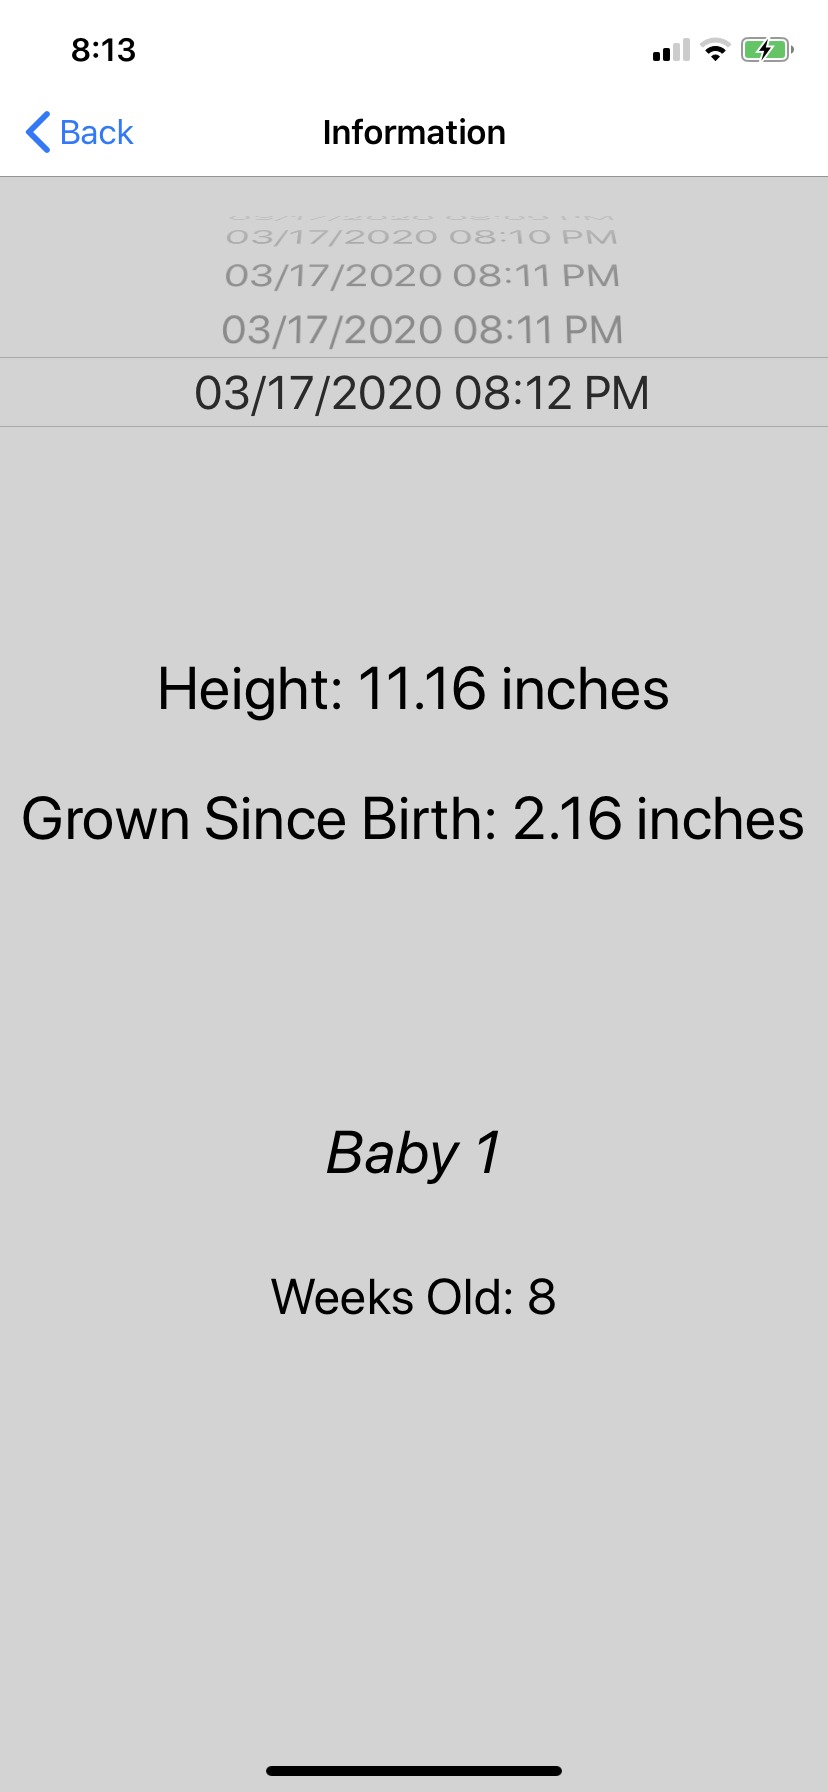
\includegraphics[width=70mm]{./images/health-info-screen.png}
\caption{Health information screen}
\end{figure}

\end{document}